% $Header: /home/vedranm/bitbucket/beamer/solutions/generic-talks/generic-ornate-15min-45min.en.tex,v 90e850259b8b 2007/01/28 20:48:30 tantau $

\documentclass{beamer}

% This file is a solution template for:

% - Giving a talk on some subject.
% - The talk is between 15min and 45min long.
% - Style is ornate.



% Copyright 2004 by Till Tantau <tantau@users.sourceforge.net>.
%
% In principle, this file can be redistributed and/or modified under
% the terms of the GNU Public License, version 2.
%
% However, this file is supposed to be a template to be modified
% for your own needs. For this reason, if you use this file as a
% template and not specifically distribute it as part of a another
% package/program, I grant the extra permission to freely copy and
% modify this file as you see fit and even to delete this copyright
% notice.


\mode<presentation>
{
  \usetheme{Warsaw}
  % or ...

  \setbeamercovered{transparent}
  % or whatever (possibly just delete it)
}


\usepackage[english]{babel}
% or whatever

\usepackage[latin1]{inputenc}
% or whatever

\usepackage{times}
\usepackage[T1]{fontenc}
% Or whatever. Note that the encoding and the font should match. If T1
% does not look nice, try deleting the line with the fontenc.


\usepackage{marvosym} % For \Smiley
\usepackage{verbatim} % for \verbatiminput

\title
{IBL \& Mathematical Puzzlehunt Competitions}

\subtitle
{Legacy of R.L.M. Conference - 2015} % (optional)

\author%[Clontz, Couch] % (optional, use only with lots of authors)
{Steven~Clontz\inst{1} \and PJ~Couch\inst{2}}%\inst{1} \and S.~Another\inst{2}}
% - Use the \inst{?} command only if the authors have different
%   affiliation.

\institute % (optional, but mostly needed)
{
  \inst{1}
  Auburn, AL
  \and
  \inst{2}
  Lamar University
}

\date[15-06-27] % (optional)
{June 27, 2015}


% If you have a file called "university-logo-filename.xxx", where xxx
% is a graphic format that can be processed by latex or pdflatex,
% resp., then you can add a logo as follows:

 % \pgfdeclareimage[height=1cm]{university-logo}{auburn_logo.png}
 % \logo{\pgfuseimage{university-logo}}



% Delete this, if you do not want the table of contents to pop up at
% the beginning of each subsection:
%\AtBeginSubsection[]
%{
%  \begin{frame}<beamer>{Outline}
%    \tableofcontents[currentsection,currentsubsection]
%  \end{frame}
%}


% If you wish to uncover everything in a step-wise fashion, uncomment
% the following command:

%\beamerdefaultoverlayspecification{<+->}


\newcommand{\vpause}{\pause\vspace{1em}}

\newcommand{\term}[1]{\textbf{#1}}




\begin{document}
% \renewcommand{\pause}{}

\begin{frame}
  \titlepage
\end{frame}

% \begin{frame}{Table of Contents}
%   \tableofcontents
%   % You might wish to add the option [pausesections]
% \end{frame}

\section{Puzzlehunts}

\subsection{About puzzlehunts}

\begin{frame}
  A \textbf{puzzlehunt} is a type of scavenger hunt which replaces
  the list of items to collect
  with a list of puzzles to solve.
\end{frame}

\begin{frame}
  EPP15: Eric's Circle of Friends (March 14, '15 9:26:53am) \\
  http://www.ericharshbarger.org

  \begin{center}
    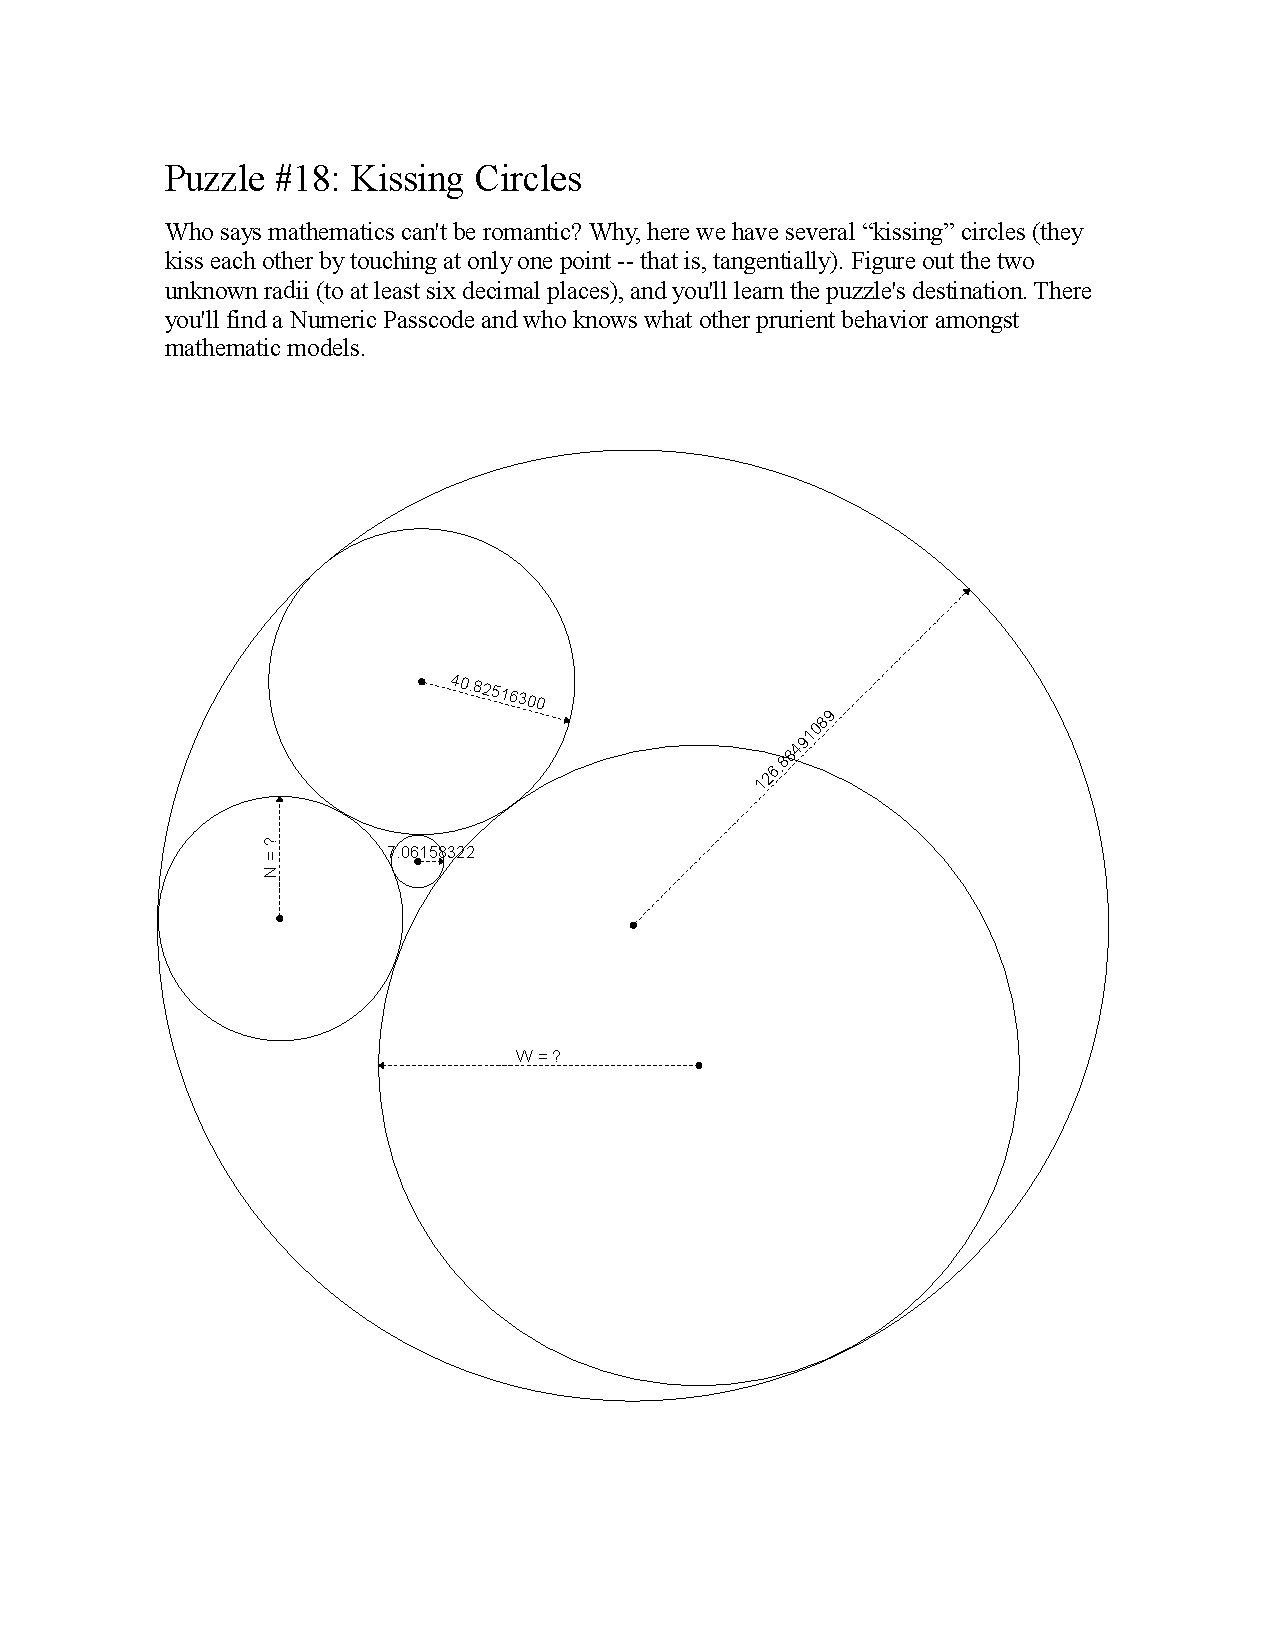
\includegraphics[height=0.8\paperheight]
    {kissing_circles.pdf}
  \end{center}
\end{frame}

\begin{frame}
  Locations where EPP15 solutions were found:

  \begin{center}
    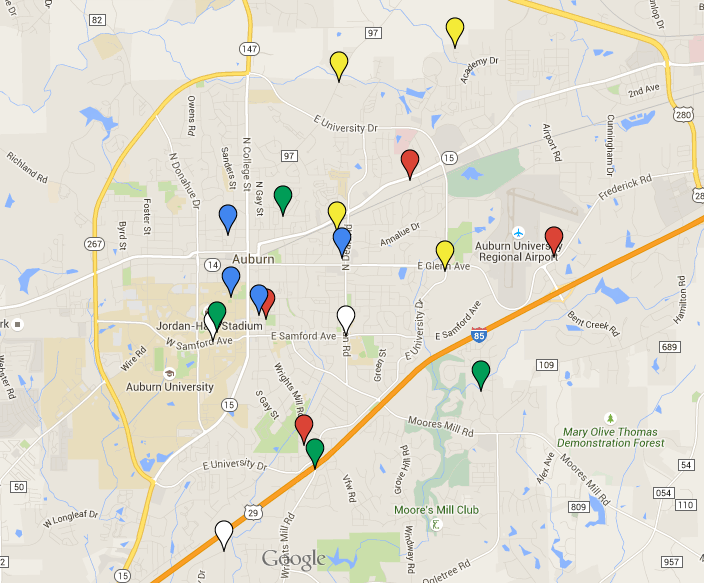
\includegraphics[height=0.7\paperheight]
    {epp15map.png}
  \end{center}
\end{frame}

\begin{frame}
  Famous puzzlehunts include:
  \begin{itemize}\small
  \item MIT Mystery Hunt
  \item Microsoft College Puzzle Challenge
  \item DASH (Different Area Same Hunt)
  \item Various ``room escape'' challenges
  \end{itemize}
  \pause

  The last two seasons of \textit{The Big Bang Theory} have featured
  episodes about puzzlehunts and room escape games.

  \vpause

  Some puzzlehunts are organized by communities of puzzle solvers,
  and others are sponsored by companies.

  \vpause

  Businesses use puzzles in interviews to determine if
  future employees are able to problem-solve.
\end{frame}

\subsection{IBL and Puzzles}

\begin{frame}
  Solving well-designed IBL coursenotes and puzzles
  are very similar processes:

  \pause

  \begin{itemize}
    \item The solution is (often) not algorithmic.
    \pause
    \item Everything is on the page for a reason.
    \pause
    \item Solutions are leading somewhere.
  \end{itemize}
\end{frame}

\begin{frame}
  Many players report added satisfaction with a puzzle if they feel like they
  learned something new along the way.

  \vpause

  Likewise, mathematical challenges should be designed like
  puzzles: to be solved, not to confound.
\end{frame}

\begin{frame}
  Posing team-based math puzzles support the
  Common Core Standards for Mathematical Practice.

  \pause

  \begin{itemize}
    \item Model with mathematics.
    \pause
    \item Make sense of problems and persevere in solving them.
    \pause
    \item Construct viable arguments and critique the reasoning of others.
    \pause
    \item Etc...
          http://www.corestandards.org/Math/Practice/
  \end{itemize}
\end{frame}

\section{Mathematical Puzzlehunts}

\subsection{AMP'd}

\begin{frame}
  AMP'd (Auburn Mathematical Puzzle) Challenge (est. 2012)
  \begin{itemize}
    \item Adaptation of Australian IBL math camp
          as single-day middle school competition
  \end{itemize}

  \vpause

  Goal: students collaborate as a team to solve puzzles by modeling them
  with mathematics.
\end{frame}

\subsection{LaMP}

\begin{frame}
  LaMP (Lamar Mathematical Puzzle) Challenge (est. 2015)
  \begin{itemize}
    \item Blend of IBL experience and puzzlehunt
  \end{itemize}

  \vpause

  Goal: encourage underrepresented (88\% identified as minority)
  students to reenvision mathematics as a fun problem-solving
  activity.
\end{frame}

\section{MaPP}

\subsection{Going national}

\begin{frame}
  Based on the positive responses we received from students and
  teachers participating in AMP'd and LaMP, our team of mathematicians
  are organizing Mathematical Puzzle Programs (MaPP) to bring similar
  unique experiences to even more campuses.

  \vpause

  Our first event will be a high school competition similar to LaMP
  to a half-dozen campuses across the country in 2016.
\end{frame}

\begin{frame}{MaPP Format (tentative)}

  \begin{itemize}
    \item
    Opening Puzzle

    A physical challenge requiring students to run around a green space
    to collect data required to solve an otherwise quick puzzle.

    \vpause

    \item
    Main Puzzles

    Teams receive a packet of mathematical puzzles. Each solution unveils
    a secret message worth points, and solving the riddle within reveals
    the hidden location of an EXTRA Puzzle.

  \end{itemize}
\end{frame}

\begin{frame}{MaPP Format (tentative)}

  \begin{itemize}
    \item
    EXTRA Puzzles

    Extensions to the main puzzles involving optimization.
    Teams which submit the best solution earn points.

    \vpause

    \item
    Metapuzzle

    An undergraduate-level mathematics problem from field underrepresented
    in HS. Points are awarded based on the
    generality of the submited solutions.
  \end{itemize}
\end{frame}

\subsection{Moving forward}

\begin{frame}
  Plans for the future...
  \pause
  \begin{itemize}
    \item Open source materials for free use in the classroom
    \vpause
    \item Build web application to manage the game and allow remote
          teams to participate
    \vpause
    \item More elaborate manipulative puzzles
    \vpause
    \item Support regional/national competitions for top teams.
  \end{itemize}
\end{frame}

\subsection{Getting Involved}
\begin{frame}
  \begin{center}\tiny
    
\includegraphics[height=10em]
    {mapp_logo_draft.jpg} \\
    (tentative logo)
  \end{center}
  \begin{itemize}
    \item \url{http://www.mappmath.org}
    \item Twitter: @StevenXClontz, @MaPPMath
  \end{itemize}
\end{frame}

\section*{}

\begin{frame}
Questions? Thanks for listening to us!
\end{frame}


\end{document}


